\documentclass{standalone}

\usepackage{amssymb}
\usepackage{amsthm}
\usepackage{amsmath}


\usepackage{tikz}
\usetikzlibrary{shapes,backgrounds,calc,patterns}


\begin{document}
	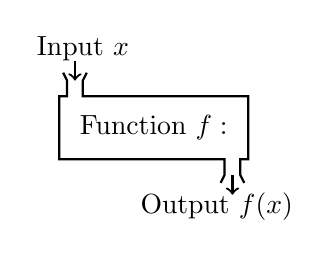
\begin{tikzpicture}
	\node at (-.9,1) {Input \(x\)};
	\node at (0,0) {Function \(f:\)};
	\node at (.8,-1) {Output \(f(x)\)};
	%\draw (-1.2,.4) rectangle (1.2,-.4);
	\draw [thick] (.85,-.7) -- (.9, -.6) -- (.9,-.4) -- (-1.2,-.4) -- (-1.2,.4) -- (-1.1,.4) -- (-1.1,.6) -- (-1.15,.7);
	\draw [thick] (-.85,.7) -- (-.9,.6) -- (-.9,.4) -- (1.2,.4) -- (1.2,-.4) -- (1.1,-.4) -- (1.1,-.6) -- (1.15,-.7);
	\draw [->, thick] (-1,.85) -- (-1,.6);
	\draw [->, thick] (1,-.6) -- (1,-.85);
	\end{tikzpicture}
	
	
\end{document}